\section{SW02}


\subsection{Testen vs Experimentieren}

Testen unterscheidet sich von Experimentieren dadurch, dass es beim Testen eine Erwartung gibt die belegt werden soll, während das Ergebnis beim Experimentieren offen ist oder nur vermutet werden kann:
\begin{itemize}
    \item Anforderungen (= erwartetes Verhalten) müssen bekannt sein
    \item Testen bedingt Anforderungen und prüft auf Unterschiede
    \item ohne Anforderungen ist Testen schwierig bis unmöglich
    \item Der Kontext vom Testen ist wichtig (Formale Nachweise, zb für Flugzeugindustrie, benötigen einen viel höheren formellen Aufwand für das selbe in einem anderen Kontext)
\end{itemize}

\subsection{Agiles Testen}

Vorteile von agilem Vorgehen:
\begin{itemize}
    \item kurze Zyklen bringen schnell Feedback
    \item CI / CD unterstützen schnelles Feedback
    \item Jede Teillieferung bringt Nutzen
    \item Wichtiges erfolgt zuerst
\end{itemize}

Gefahren bei agilem Vorgehen:
\begin{itemize}
    \item Ganzheitlicher (Test-) Ansatz fehlt (= keine Teststrategie)
    \item Keine Negativ-Tests
    \item Keine Grenzwerttests
    \item Keine NFA – Tests (Nicht Funktionale Anforderungen)
    \item Automatisierung erfolgt zu spät weil Produkt zulange instabil ist
\end{itemize}

Aus Test Sicht wichtige Punkte welche Aufmerksamkeit benötigen beim agilen Vorgehen:
\begin{itemize}
    \item PO hat (zu) grosse Verantwortung (und oft wenig bis kein Testwissen)
    \item Ein Team kann «Alles», jede und jeder im Team können «Alles»
    \item Es gibt Akzeptanzkriterien (AK)
    \item Es gibt eine DOD (Definition of Done) und teilweise eine DOR (Definition of Ready: Wenn die Product Backlog Items "ready" für den Sprint sind~\cite{scrum-events.de})
    \item Es darf / muss Teststories\footnote{Teststory ist ein Bestandteil einer User Story. Weiter Bestandteile können sein: Technical Story, Infrastructure Story, ...} geben, diese beinhalten folgende Tätigkeiten:
    \begin{itemize}
        \item Codereview
        \item Testanalyse (Was muss getestet werden)
        \item Testdesign (Wie wird getestet, wie sieht der Testablauf aus)
        \item Tests bauen (auch automatisierte)
        \item Testdaten (Passende, realistische Testdaten definieren und bereitstellen)
        \item Tests durchführen
    \end{itemize}   
\end{itemize}

\subsection{Rollen/Tätigkeiten im Testing}

Abbildung \ref{fig:Rollen im Testing} zeigt einen Vorschlag von möglichen Rollen mit den jeweiligen Verantwortlichkeiten und notwendigen Skill Set.

\begin{figure}
\centering
\begin{minipage}{.47\textwidth}
  \centering
  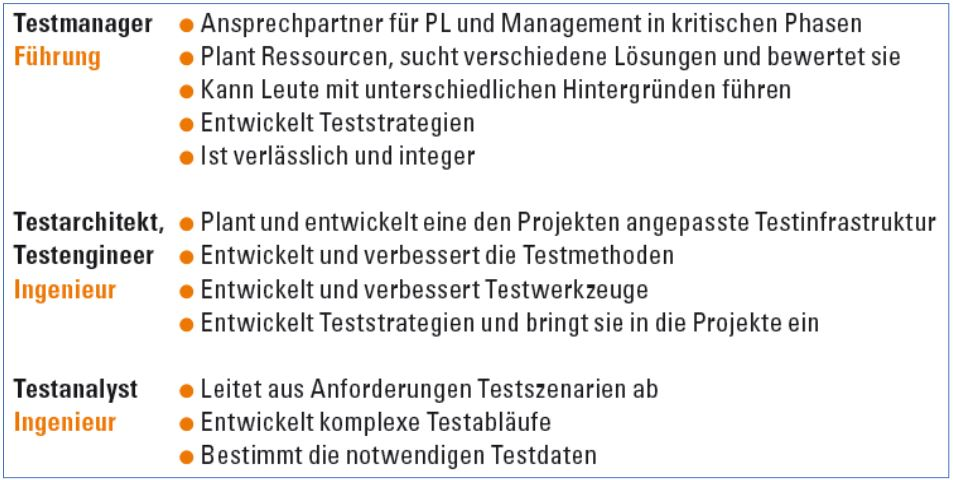
\includegraphics[width=1\linewidth]{02/bilder/Taetigkeiten Testing 1.JPG}
\end{minipage}%
\begin{minipage}{.53\textwidth}
  \centering
  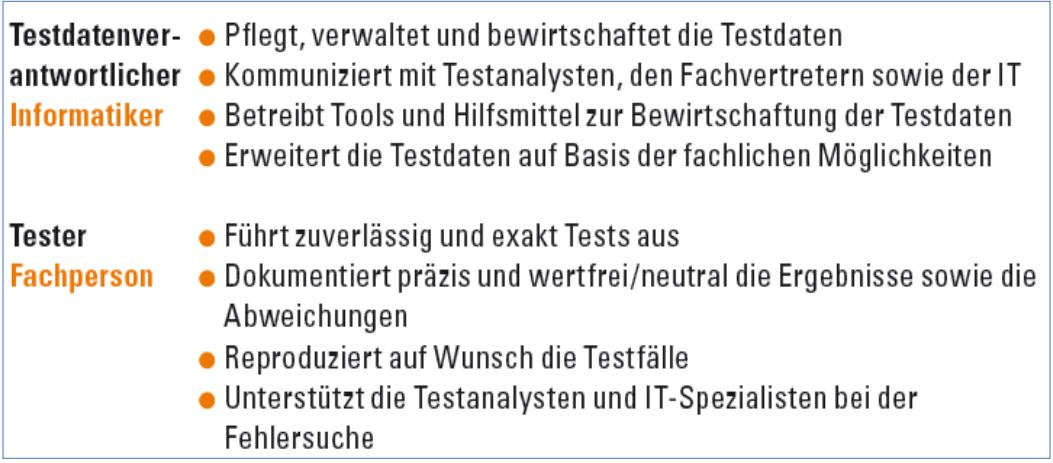
\includegraphics[width=1\linewidth]{02/bilder/Taetigkeiten Testing 2.JPG}
\end{minipage}
	\caption{Vorschlag von 5 möglichen Rollen/Tätigkeiten im Testing.}
	\label{fig:Rollen im Testing}
\end{figure}

\subsection{Test-Prozess}

Prozesse definieren Abläufe, Rollen und Verantwortlichkeiten klären. Orientiert man sich beim Testen an einem Prozess, wird sichergestellt, dass Tests:
\begin{itemize}
    \item geplant
    \item vorhersehbar
    \item gesteuert
    \item nachvollziehbar
    \item systematisch
\end{itemize}
sind. Es soll dabei beachtet werden das der Prozess nur ein Hilfsmittel ist. Beispiel: Zertifizierte Schwimmwesten aus Beton sind zwar nach Prozess erzeugt, jedoch überhaupt nicht zweckmässig. Abbildung \ref{fig:Einordnung Testprozess} zeigt eine Übersicht, wo der Testprozess einzuordnen ist.

\begin{figure}[H]
	\centering
	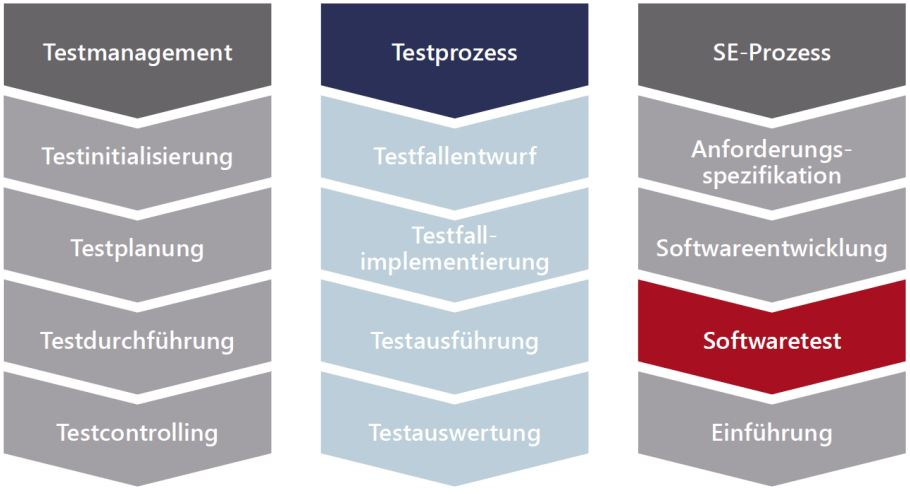
\includegraphics[width=0.7\columnwidth]{02/bilder/Einordnung Testprozess.JPG}
	\caption{Übersicht, wo der Testprozess in der Software Entwicklung (SE) Einzuordnen ist.}
	\label{fig:Einordnung Testprozess}
\end{figure}

Nachfolgend in Abbildung \ref{fig:Phasen des Testings} sind die vier Phasen des Testen's gezeigt.

\begin{figure}
    \centering
    \begin{minipage}{.48\textwidth}
        \centering
        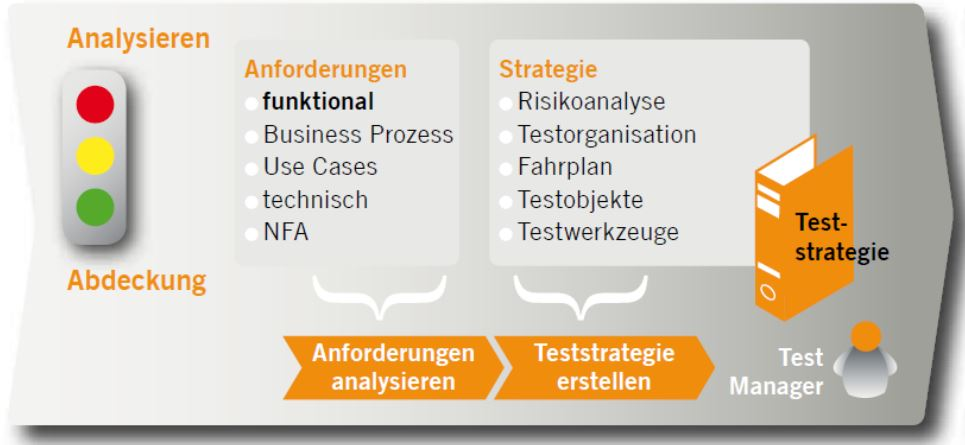
\includegraphics[width=1\linewidth]{02/bilder/Testprozess1.JPG}
        \caption{Phase 1: Analysieren.} 
        \vspace{2ex}
    \end{minipage}
    \begin{minipage}{.48\textwidth}
        \centering
        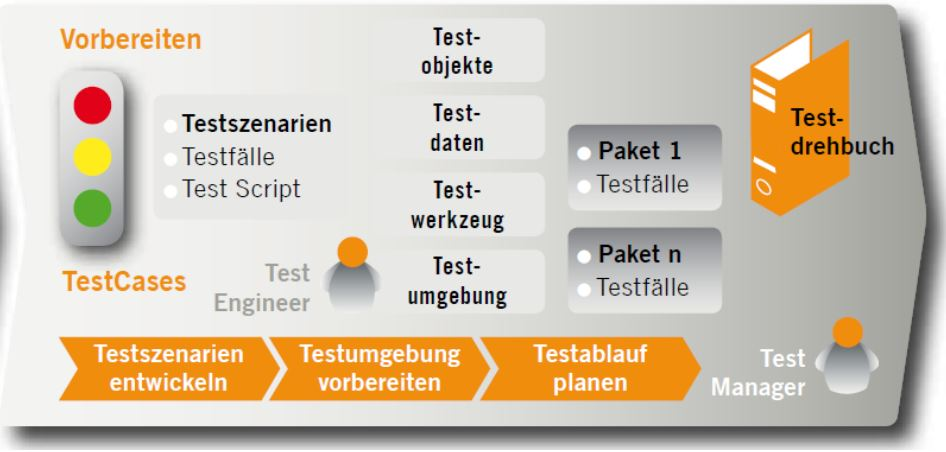
\includegraphics[width=1\linewidth]{02/bilder/Testprozess2.JPG}
        \caption{Phase 2: Vorbereiten.} 
        \vspace{2ex}
    \end{minipage}
    \begin{minipage}{.48\textwidth}
        \centering
        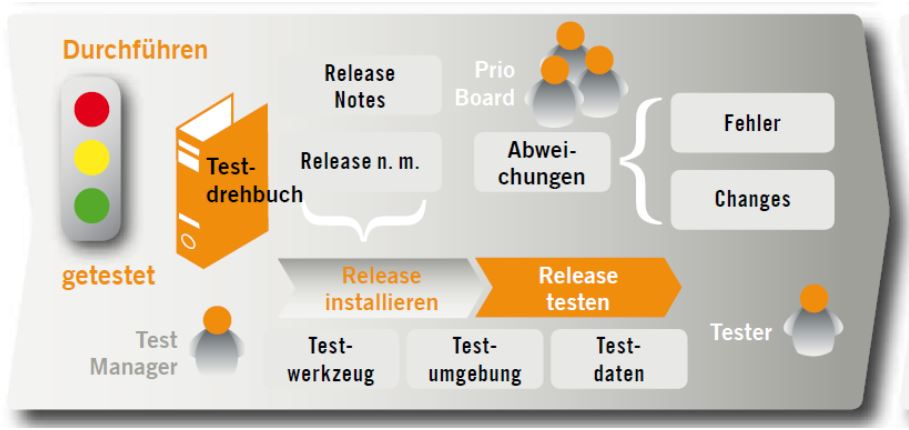
\includegraphics[width=1\linewidth]{02/bilder/Testprozess3.JPG}
        \caption{Phase 3: Durchführen.} 
        %\vspace{4ex}
    \end{minipage}
    \begin{minipage}{.48\textwidth}
        \centering
        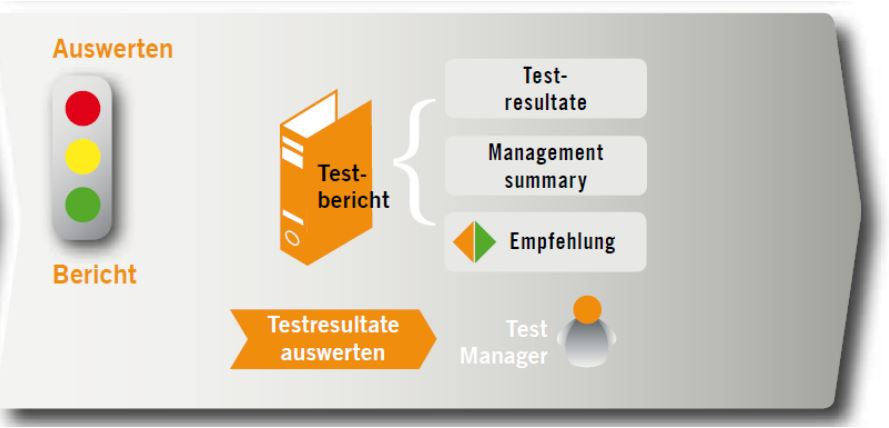
\includegraphics[width=1\linewidth]{02/bilder/Testprozess4.JPG}
        \caption{Phase 4: Auswerten.} 
        %\vspace{4ex}
    \end{minipage}
	\caption{Die 4 Phasen des Testprozesses von Noser~\cite{theNoserWayOfTesting}.}
	\label{fig:Phasen des Testings}
\end{figure}

\subsection{Testprozess, Phase 1: Analysieren}

Abbildung \ref{fig:Testprozess Phase 1} zeigt die Details in Phase 1.

\begin{figure}[H]
	\centering
	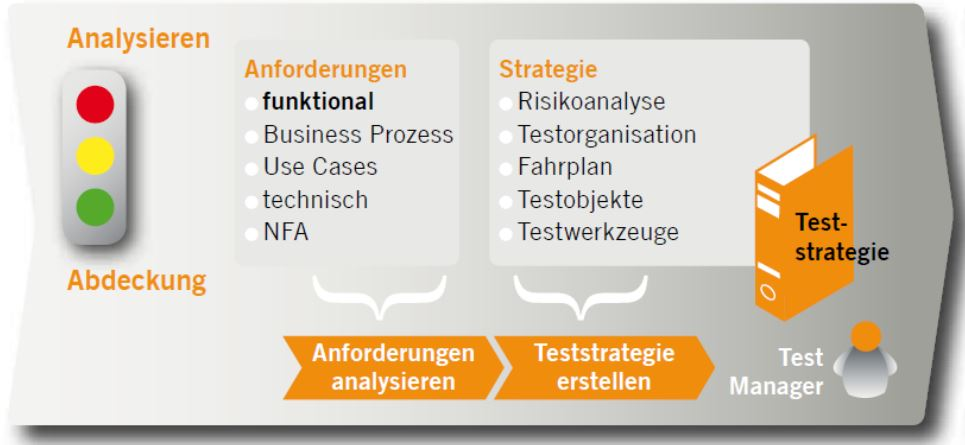
\includegraphics[width=0.8\columnwidth]{02/bilder/Testprozess1.JPG}
	\caption{Phase 1: Abdeckung Analysieren.}
	\label{fig:Testprozess Phase 1}
\end{figure}

\subsection{Teststrategie}
Grundsätzlich bestimmt eine Teststrategie, ob, was und wie tief getestet werden soll. Die Teststrategie bestimmt das Test-Ziel und weist dessen Nutzen aus. Mit der Teststrategie setzt man Prioritäten, welche Bereiche wichtig sind zu testen. Prioritäten setzt man, da man weder unendlich Zeit noch unendlich Geld hat.

Aus folgenden Fragen kristallisiert sich die Teststrategie:
\begin{itemize}
    \item Was kann im Fehlerfall passieren? (Menschenleben, Gesundheit, Umwelt, Reputation)
    \item Frage der Haftung und Garantie? (Nach EU Recht hat man 2 Jahre Garantie auf SW!)
    \item Wie lange «lebt» das Projekt / Produkt?
    \item In welchem Umfeld wird es eingesetzt? (Bsp: Billetautomaten Regen + Touch Screen / Sonneneinfall + Sichtbarkeit von Screen)
    \item Wie «komplex» ist das Produkt?
    \item Was kostet das Produkt? (Testen muss im Verhältnis sein zum erwarteten Umsatz)
    \item Gibt es Gesetze , Vorschriften oder Normen? (Datenschutz) (Kann man typischerweise nur mit Tests belegen)
    \item Welchen «Standard» haben vergleichbare Produkte? (tieferer Standart als die Konkurrenz erschwert den Markteinstieg)
    \item In welcher «Liga» wird das Produkt lanciert? (Budget vs Premium)
    \item Wie «sicher» soll oder muss das Produkt sein?
\end{itemize}

\subsection{Übung: Test-Strategie in 15 Minuten}

Abbildung \ref{fig:Teststrategie in 15 min} zeigt eine Hilfestellung um eine Test-Strategie in 15 Minuten zu entwickeln.

\begin{figure}[H]
	\centering
	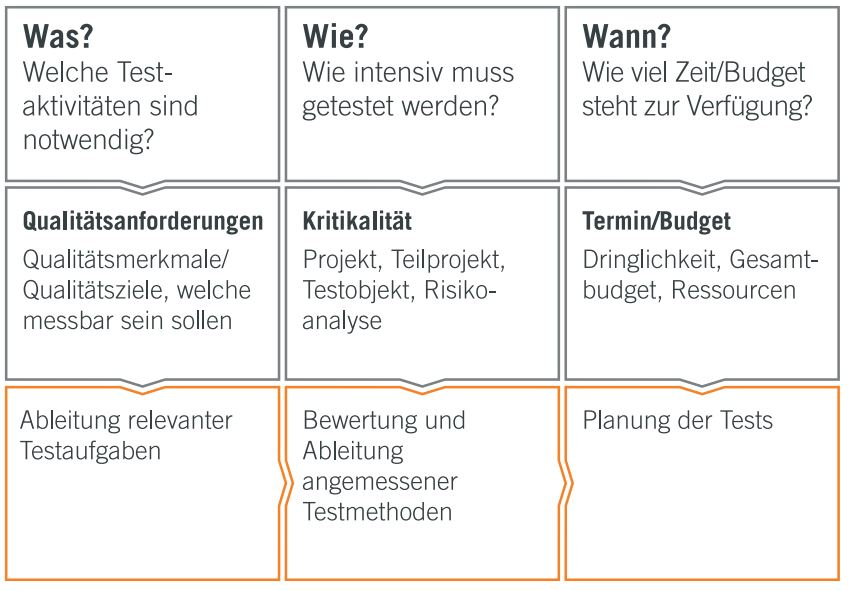
\includegraphics[width=0.6\columnwidth]{02/bilder/Teststrategie in 15 min.JPG}
	\caption{Hilfestellung für eine Test-Strategie in 15 Minuten~\cite{theNoserWayOfTesting}.}
	\label{fig:Teststrategie in 15 min}
\end{figure}

Beispiel Teststrategie für Game:
\begin{itemize}
    \item Welche Testaktivitäten sind notwendig? Das Spiel soll flüssig (NFT) und ohne Game Play beeinträchtigende Fehler spielbar sein. Daraus sind folgende relevanten Testaufgaben abgeleitet:
    \begin{itemize}
        \item Performance Test auf handelsüblichen Geräten
        \item Game Play Tests (Alpha /Beta Tests) um allfällige Fehler zu finden
    \end{itemize}
    \item Wie intensiv muss getestet werden? Das Risiko ist sehr tief, einzig die Gefahr besteht das aufgrund von zu vielen Fehlern die Motivation zum entwickeln reduziert.
    \begin{itemize}
        \item Beim entdecken von Bugs zuerst Tests schreiben welche diese Bugs Beschreiben und Ihn und ähnliche Bugs entdecken
        \item Komplizierte Konzepte und Anordnungen vorgängig (TDD) testen, da man sicher sein kann, viele Bugs im Code zu haben
    \end{itemize}
    \item Wie viel Zeit/Budget steht zur Verfügung? Da dies ein Freizeit Projekt ist, hat man weder Zeit noch Geld. Die einzig verfügbare Ressource ist die Motivation, welche die resultierende Zeit bestimmt. Eine hohe Motivation kommt von einem Funktionierenden Prototypen und neuen Features.
\end{itemize}